\documentclass{book}
\usepackage[utf8]{inputenc}
\usepackage[T1]{fontenc}
\usepackage[brazilian]{babel}
\usepackage[publish]{coop-writing}
\usepackage{indentfirst} 
\setlength{\parskip}{.5em}
\usepackage{multirow}
\usepackage{booktabs}
\usepackage{enumitem}
\usepackage{graphicx}
\usepackage[scale=5]{ccicons}
\usepackage{draftwatermark}
\SetWatermarkText{DRAFT}
\SetWatermarkScale{5}
\setlist{nosep}
\usepackage[natbib,style=authoryear]{biblatex}
\addbibresource{luderia.bib}
\usepackage{outlines}
\usepackage{hyperref}
\cwnamedef{rafael}{blue}{Rafael}
\cwnamedef{xexeo}{red}{Xexéo}
\usepackage{titling} % construir página de title
\predate{\centering}
\postdate{\vfill\hfill\ccbyncsa\hfill}

\title{\Huge Luderia}
\author{\Large Geraldo Xexéo \\
com a colaboração de Rafael Monclair}
\date{June 2021}

\begin{document}

\frontmatter



\maketitle
\tableofcontents
\chapter*{Licença}

\begin{center}
\ccbyncsa    

\vspace{1cm}

Este texto é distribuído com uma licença Creative Commons - Atribuição - NãoComercial - CompartilhaIgual 4.0 Internacional.

\end{center}






\section*{Você tem o direito de:}
\begin{itemize}
\item \textbf{Compartilhar} -- copiar e distribuir o material em qualquer suporte ou formato.
\item \textbf{Adaptar} -- remixar, transformar, e criar a partir do material.
\end{itemize}

\section*{De acordo com os termos seguintes:}
\begin{itemize}
\item \textbf{Atribuição} -- Você deve dar o crédito apropriado, prover um link para a licença e indicar se mudanças foram feitas. Você deve fazê-lo em qualquer circunstância razoável, mas de nenhuma maneira que sugira que o licenciante apoia você ou o seu uso.
\item \textbf{NãoComercial} --Você não pode usar o material para fins comerciais.
\item \textbf{CompartilhaIgual} -- Se você remixar, transformar, ou criar a partir do material, tem de distribuir as suas contribuições sob a mesma licença que o original.
\item \textbf{Sem restrições adicionais} -- Você não pode aplicar termos jurídicos ou medidas de caráter tecnológico que restrinjam legalmente outros de fazerem algo que a licença permita.
\end{itemize}

Mais informações podem ser encontradas em \url{https://creativecommons.org/licenses/by-nc-sa/4.0/deed.pt_BR}

\mainmatter

\chapter{Introdução a Luderia}
\label{chap:intro}

Uma luderia é uma loja que aluga e vende jogos. Normalmente, esse tipo de negócio inclui um bar ou restaurante, que atende os fregueses, monitores que ensinam a jogar e possivelmente outras atividades. 

O aluguel de jogos é basicamente um diferencial de atração, não sendo a única fonte de renda, que é o consumo no bar e restaurante. Porém, ele também tem que dar lucro, além de exigir um trabalho de curadoria e monitoria, como veremos neste documento.

Esse documento descreve o funcionamento da Luderia SemNome, que é feito todo de forma manual, usando papel e caneta. A suposição é que todo serviço será informatizado, em vários módulos que comporão um sistema único.

Basicamente, uma luderia pode funcionar com diferentes modelos de negócio: cobrar ingresso, cobrar consumo mínimo, cobrar pelo aluguel dos jogos, ou um mix desses modelos. A Luderia SemNome trabalha com o modelo de ingresso, mas quer ter liberdade para mudar esse modelo em qualquer momento, ou variar o modelo por dia.

Este documento serve de referência para exercícios de Engenharia de Software, da especificação de serviço ao desenvolvimento, teste e manutenção, de um sistema de informação que apoia todas as suas funções de negócio.

\section{Serviços prestados na Luderia}

A Luderia SemNome oferece os seguintes serviços, que serão tratados de forma detalhada mais adiante no texto:
\begin{enumerate}
    \item uma recepção (Capítulo \ref{chap:recepcao});
    \item empréstimo (Capítulo \ref{chap:aluguel}), no local, de jogos de tabuleiro e cartas;
    \item atendimento com bebidas (Capítulo \ref{chap:barest}), incluindo refrigerantes, bebidas alcoólicas, drinks com ou sem álcool e sucos naturais, feitas no bar;
    \item atendimento com comidas (Capítulo \ref{chap:barest}), incluindo lanches, como sanduíches e pizza, aperitivos, como porções de batata-frita, pratos feitos, como filé com fritas, feitas na cozinha;
    \item garçons ou \textit{self-service} (Capítulo \ref{chap:barest}), conforme a escolha do cliente;
    \item uma grande área com mesas onde se pode jogar ou consumir alimentos e bebidas;
    \item monitoria (Capítulo \ref{chap:monitor}), com monitores que ensinam a jogar os jogos, e a ainda outras formas de apoio ao jogador, como mestres cadastrados e professores;
    \item um clube de membros (Capítulo \ref{chap:clube});
    \item uma loja (Capítulo \ref{chap:loja}), onde se podem comprar jogos de tabuleiro e cartas, além de acessórios;
    \item aluguel de jogos, que permite que o cliente leve o jogo para casa;
    \item um setor de entregas, que entrega comidas e jogos, emprestados ou vendidos;
    \item um caixa único, na saída da Luderia;
    \item a gerência de RH, responsável pelo pessoal;
    \item a gestão financeira, que controla o resultado;
    \item o estoque da loja (Capítulo \ref{chap:loja});
    \item o estoque de empréstimos, que fica localizado em uma parede da loja, e
    \item o estoque de bebidas e alimentos, prontos ou insumos.
    \rafael{ Não sei se valeria incluir a pessoa responsável por lidar com as editoras para comprar jogos novos.}
\end{enumerate}


\section{Horário de Funcionamento e Cobrança}

Os horários de funcionamento da Luderia e como é cobrado o ingresso, estão descritos na Tabela \ref{tab:ludehorarios}. Detalhes da forma de aluguel atual e planos para o futuro são descritos no Capítulos \ref{chap:aluguel}. Os horários podem mudar no futuro.

\begin{table}[hbt]
    \centering
    \begin{tabular}{cccc}
    \toprule
    dia & início & fim & cobrança\\
    \midrule
        segunda & \multicolumn{3}{c}{não funciona} \\
         terça & 13:00 & 22:00 & ingresso grátis \\
         quarta e quinta & 13:00 & 22:00 & ingresso com desconto cobrado 50\%\\
         sexta e sábado & 12:00 & 24:00 & ingresso normal \\
         domingo & 12:00 & 21:00 & ingresso normal \\
    \bottomrule
    \end{tabular}
    \caption{Horários da Luderia}
    \label{tab:ludehorarios}
\end{table}

\section{Como é a Luderia}

A Luderia tem como espaço físico uma grande casa de três andares, que permite dividir de forma adequada os serviços, de acordo com o seguinte quadro:
\begin{itemize}
    \item hall, onde estão 3 balcões: recepção, balcão de empréstimos e caixa;
    \item loja, em um salão no térreo acessado pelo hall;
    \item salas de mesa, uma sala no primeiro e duas segundo andar;
    \item um salão para reservas, dedicado a festas ou eventos privados, no terceiro andar;
    \item ludoteca, uma pequena sala no primeiro andar com estantes com jogos e uma mesa para permitir que os clientes os abram, além de um balcão de aluguel. \rafael{ No caso da Ludus, que é a maior que conheço, isso fica numa vitrine, mas o cliente não toca nisso. Ele pode até apontar e pedir para um monitor pegar, mas quem manuseia e lida com os jogos antes de irem pra mesa é o monitor.}
    \item bar, um balcão grande no primeiro andar, que permite fazer drinks e sucos, e um balcão de apoio no segundo andar;
    \item cozinha, no primeiro andar;
    \item banheiros, masculino e feminino, no primeiro e segundo andares;
    \rafaelx{ A Game of Boards aboliu os gêneros. Agora os banheiros são mistos.}
    \item gerência, vestiário, banheiros dos funcionários, no terceiro andar, e 
    \item um depósito, em uma outra construção fora da casa.
    \end{itemize}

Uma escada liga todos os andares. Não há elevador, porém a escada possui um dispositivo que permite que uma pessoa com dificuldades se sente e seja levado.

Só é possível sair da Luderia passando pela loja. Existe um elevador de alimentos da cozinha para o segundo andar, mas não para o terceiro.

\begin{figure}[hbt]
    \centering
    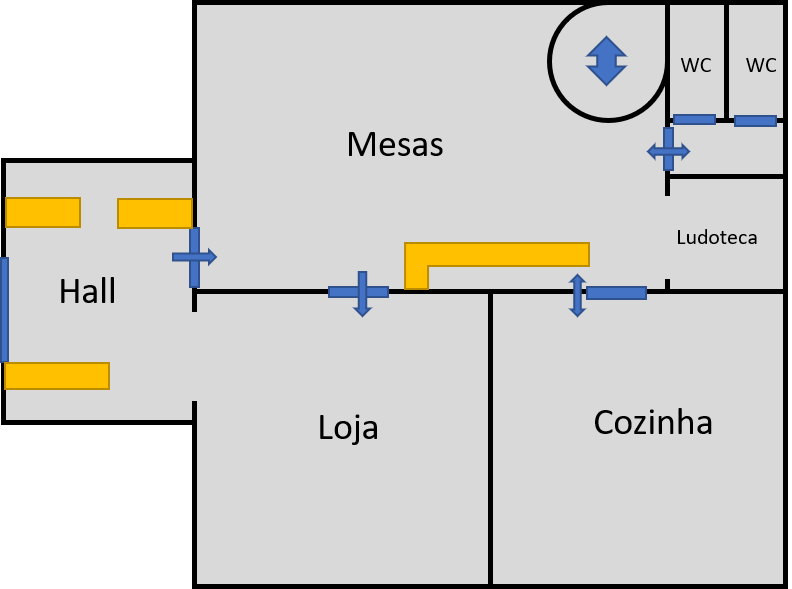
\includegraphics[scale=0.8]{imagens/PrimeiroAndar.png}
    \caption{Primeiro andar da Luderia}
    \label{fig:andar1}
\end{figure}

\begin{figure}[hbt]
    \centering
    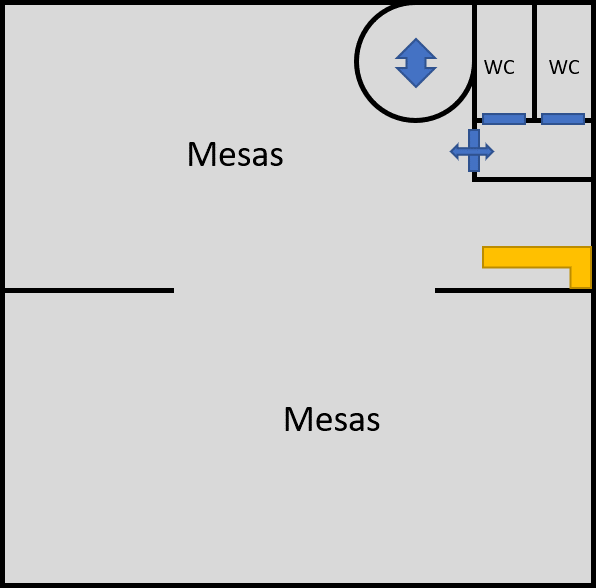
\includegraphics[scale=0.8]{imagens/SegundoAndar.png}
    \caption{Segundo andar da Luderia}
    \label{fig:andar2}
\end{figure}

\begin{figure}[hbt]
    \centering
    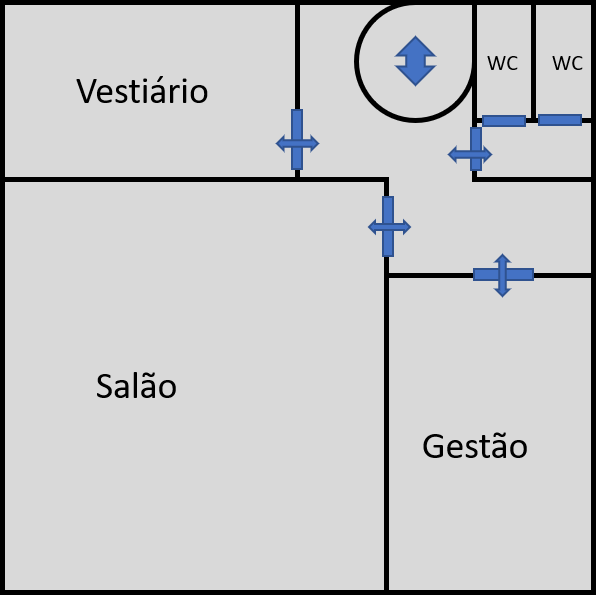
\includegraphics[scale=0.8]{imagens/TerceiroAndar.png}
    \caption{Terceiro andar da Luderia}
    \label{fig:andar3}
\end{figure}

\section{O atendimento atual}

O atendimento atual é todo feito na mão, com um cartão de consumo de papel onde os funcionários anotam as compras.

Esse cartão traz vários problemas. Se perdido, não se sabe quanto a pessoa consumiu. Os funcionários têm letra ruim, dificultando a vida do caixa.

Eles ainda amassam, molham e devem ser impressos frequentemente, ou guardados, se impressos em grande quantidade.


\section{O cartão de consumo de plástico}

A empresa decidiu que o sistema deverá usar um cartão de consumo de plástico, e já os comprou.

O cartão de consumo a ser usado contém um número e um QR-Code que representa esse número. Todos os funcionários da Luderia carregarão um equipamento (mini-tablet) que permitirá usar o sistema a ser construído para registrar pedidos na conta do cliente, bastando para isso scannear o cartão ou usar o número que está nele impresso.
\rafaelx{ Diria que esse número é em alto relevo, caso contrário, com o manuseio, o QR code e os dígitos ficarão desgastados.}

A Luderia comprou um pacote de 1000 cartões, mesmo que não caibam tantas pessoas na casa.

\section{A questão do barulho, brigas e assédio}

A Luderia é destinada a jogos de sociedade que fazem barulho naturalmente. Jogos que exigem silêncio podem ser jogados, quando disponível, isto é, não estiver sendo alugado, no salão do terceiro andar. Nesse caso, o comportamento no local deve ser de máximo esforço para o silêncio, sendo apenas permitidas conversas exigidas pelo jogo.

Barulho excessivo, porém, poderá ser controlado pelos monitores. Brigas serão imediatamente interrompidas pelo monitor responsável pela sala. A violência física significa o banimento do jogador da Luderia. Deve haver registro do jogador banido em qualquer sistema futuro.

O assédio moral e sexual também é causa de banimento.

\section{Proibições e Permissões}

Não é permitido o jogo com apostas. 

Em geral, também não é permitido trazer bebidas e comidas de fora, sendo que exceções são feitas para alimentação de crianças pequenas.

Grupos trazem seu próprio jogo estão sujeitos a pagar a consumação mínima, ou pagar a taxa de aluguel de jogos mais baratos, dependendo da forma de cobrança. Se a cobrança for por ingresso, isto não será necessário.

\section{Pedidos gerais sobre a implementação}

O sistema informatizado deve ter as seguintes características, segundo os proprietários:
\begin{itemize}
    \item ser um sistema único e integrado;
    \item usar uma base de dados open-source, gratuita e única;
    \item ter uma interface de usuário com programação única, via web, e que se adapte aos vários dispositivos que vão ser usados, podendo ser acessado via: celulares, tablets e computadores, como telas de diferentes tamanhos;
    \item parte do sistema deverá ser acessada diretamente pelos clientes;
    \item ter uma interface com serviços de emissão de nota fiscal, e
    \item usar linguagens de programação gratuitas e abertas.
\end{itemize}

\rafael{ O que você acha dos membros cadastrados na plataforma, mesmo que não paguem mensalidade, poderem consultar antecipadamente se um determinado jogo está na loja, antes da pessoa ter que se deslocar até lá.}


\chapter{Recepção}
\label{chap:recepcao}

As funções da recepção são:
\begin{itemize}
    \item receber os clientes;
    \item indicar a loja, o setor de empréstimo, o setor de aluguel, restaurante e mesas, conforme o interesse do cliente, e
    \item registrar o cliente que vai para as mesas, fornecendo um cartão de consumo, e avisando do consumo mínimo, quando houver.
\end{itemize}

\section{Recepção dos clientes}

A recepção dos clientes visa deixá-los mais à vontade na Luderia. Além disso, ela procura contar todos os clientes que entram e, se possível, cadastrá-los. O recepcionista tem como função conseguir o cadastro.

Para isso é necessário que haja um terminal na recepção que permita:
\begin{enumerate}
    \item simplesmente indicar a entrada de um ou mais clientes;
    \item cadastrar um cliente, e
    \item associar um cliente a um cartão de consumo.
\end{enumerate}

\section{O Cartão de Consumo}

Ao entrar na Luderia o cliente recebe um cartão de consumo, que é obrigatório. 

Só é possível consumir nas mesas com um cartão de consumo. 
Não é possível entrar na área de mesas sem um cartão. Isso é garantido por uma roleta de acesso, em horários mais cheios controlada por um segurança, enquanto em horários mais vazios é observada pelo funcionário da recepção.

Na loja e na seção de empréstimo o cartão pode ou não ser usado. Se não for usado, o cliente que comprar ou emprestar algo vai receber um cartão de consumo para pagar suas compras. 

\section{Consumo Mínimo}

Em alguns momentos, os gerentes podem decidir, que além, ou no lugar, do ingresso haverá um consumo mínimo, ou \textit{ingresso reembonsável com compras}, por exemplo, sábado entre 17:00 e 23:00 horas. Cabe a recepção avisar desse valor, porém será dado 15 minutos de perdão, isto é, se a pessoa sair em menos de 15 minutos e seu cartão estiver vazio, não precisa pagar o consumo mínimo.

\section{Registro de entrada}

O registro de entrada é feito como em boates e prédios: identificação com nome, telefone e foto em câmera portátil. O cliente deve, pelo menos, dar um nome ou apelido para o cartão de consumo. Não serão permitidos apelidos considerados ofensivos ou preconceituosos.

\section{Funcionários}

A recepção usa pelo menos um funcionário dedicado a todo momento. Esse funcionário pode cumprir outros papéis, como emprestar jogos no balcão de empréstimo ou realizar a venda de um produto da loja.

De sexta às 15 horas até domingo às 21:00 a recepção fica com 2 funcionários. Nos outros horários, fica com 1 funcionário.

A recepção atualmente tem 4 funcionários alocados a ela, que se revesam para  trabalhar, de acordo com horários pré-estabelecidos: Rui Regente, Rita Ramos, Renata Rilleti, e Rosa Raposo. Os gerentes também costumam passar algum tempo por semana na recepção. Se necessário, um caixa ou um vendedor da loja também pode cobrir a posição. 

\rafaelx{ Vamos dizer que gerentes, caixas e garçons podem ser monitores também, ou eles serão exclusivamente monitores? Na Ludus eles tinham essa distinção. Na GoB tinham e depois misturou um pouco. Mas o gerente da GoB também explicava os jogos, embora não fosse formalmente um monitor, por exemplo.}
\chapter{Empréstimo e Aluguel de Jogos}
\label{chap:aluguel}

O negócio de emprestar jogos para jogar no local é o principal chamariz da Luderia. Ele possui uma extensa coleção e mantém um registro de uso que permite analisar se mais cópias precisam ser compradas ou repostas.

Com a pandemia, a Luderia lançou o empréstimo de jogos, que podem ser retirados pelos clientes, ou entregues a eles, para jogar em casa.

Deve ficar claro que é usado o termo empréstimo para jogar na luderia e aluguel para levar para casa.

\section{O Ingresso}

A Luderia trabalha com o modelo de negócios baseado em ingresso pago, como foi apresentado no Capítulo \ref{chap:intro}

Esse modelo permite descontos, que é utilizado hoje em alguns dias, ou bônus no consumo, funcionando como um consumo mínimo, que não é usado atualmente mas é usado em algumas promoções.


\section{O Aluguel}
\rafaelx{ Por hora?! Por dia não seria melhor?}
\rafaelx{ Será que não podemos incluir um custo de depreciação? Depois de X vezes jogado/alugado ele vai ficando mais barato?}

Atualmente, os jogos são alugados por dia. É usado um  código de cores. Assim o jogo \textit{Dooble}, que é barato, é alugado com um código verde, \textit{War} na faixa amarela,  \textit{Twilight Struggle} na faixa vermelha e o \textit{Twilight Imperium: Fourth Edition} na faixa negra. 

O cálculo feito pelos donos inclui o estado do jogo, o valor do jogo no mercado, o tempo médio de partida e até uma visão de que certos jogos são jogados por pessoas que consomem mais e a chance do jogador alugar outro jogo. 


\rafaelx{ Gloomhaven tem campanhas que podem ser mais rápidas que uma partida de TS. O ideal era falar que faixa preta é o Twilight Imperium: Fourth Edition que pode durar de 4 a 8 horas e o Gloomhaven poderia até ser um faixa vermelha pra não ter dois jogos com Twilight no nome.}

Extensões são cobradas a parte, porém em alguns jogos a Luderia já inclui a expansão no valor do aluguel. Esse é o caso do \textit{Dixit}, por exemplo, que está na faixa amarela, mas uma expansão pode ser escolhida pelos jogadores como brinde.

A Luderia deseja ter possibilidades mais amplas de dar preço ao jogo, misturando um modelo por faixas, possivelmente por cores ou outro símbolo, com um modelo por preço de aluguel individual por jogo, e ainda preços por pacotes pré comprados, e preços por dia.

Além disso, a Luderia, também pretende ter descontos para associados ou frequentadores e sistemas de fidelidade, como o décimo jogo alugado ser de graça.

Jogos que vão envelhecendo ou sendo menos alugados também vão ficando mais baratos, mudando de faixa.

\section{O Cardápio de Jogos}

Já existe um cardápio de jogos impresso, mas feito artesanalmente. Esse cardápio deve ser automatizado, por meio de um site web e também de um app, e incluir, para cada jogo:
\begin{itemize}
    \item nome;
    \item descrição;
    \item nota no BGG;
    \item nome dos monitores que sabem jogá-lo;
    \item tempo médio;
    \item número de jogadores de acordo com o jogo;
    \item número recomendável de jogadores.
\end{itemize}

No futuro outras informações podem ser necessárias.

\section{Pegando o Jogo Emprestado}

Para jogar um jogo na luderia, o cliente deve mostrar o seu cartão de consumo a um monitor, que usará o sistema para associar o jogo ao jogador, informação útil para a gestão do negócio.

\rafaelx{ Caramba! Não tinha pensado nesse estilo de aluguel não. Isso é um sistema muito puxado. Particularmente, não acho maneiro. O aluguel que tinha pensado era pra pessoa levar o jogo pra casa, tipo videolocadora. Foi isso que as luderias passaram a fazer pra sobreviver durante a pandemia. O grande negócio que uma luderia como a Ludus, GoB e Boards \& Burgers (atual LudoGrill) vende e ganha em cima é a cozinha. Ter os jogos é apenas o diferencial pra galera ficar mais tempo lá dentro consumindo.}

Quem pega emprestado não é obrigado a rearrumar as peças na caixa. Eles podem deixar tudo na mesa, ou podem colocar sem ordem na caixa. Isso é função do monitor.

\rafaelx{ Ok. Entendi o que vc fez, mas aí é melhor inverter. Nos dias mais movimentados, queremos uma rotatividade maior, então é melhor expulsar logo as pessoas de lá. Nos dias mais vazios vc pode pagar um ingresso fixo e ficar lá dentro.
Existe outra modalidade que é usada no sábado: o ingresso. Nessa modalidade o jogador entra na Luderia e joga quanto quiser, pagando um ingresso fixo. }

\subsection{Outras formas previstas no futuro}

Há interesse que no futuro possam existir várias formas de empréstimo dentro da loja, de maneira a ficar em dia com o mercado. Basicamente, a Luderia quer poder optar por modelos diferentes, conforme o movimento diário. 

Os modelos a ser suportados no futuro seriam:
\begin{itemize}
\item sem ingresso
\begin{itemize}
    \item empréstimo por jogo, por tempo, por preço único;
    \item empréstimo por jogo, por tempo, por faixa de preço;
    \item empréstimo por jogo, por tempo, com valor diferenciado por jogo;
    \item empréstimo por jogo, por tempo, com faixas e valores diferenciados para alguns jogos;
    \end{itemize}
    \item com ingresso e variações;
    \begin{itemize}
    \item ingresso simples, com empréstimo à vontade;
    \item consumação mínima, incluindo ou não o modelo de empréstimo por jogo;
    \item ingresso com desconto se a consumação for maior que certo valor, por exemplo, ingresso de R\$10  que é perdoado se consumir R\$30;
\end{itemize}
\end{itemize}

%\section{Jogos de Carta}

\rafaelx{ Faz diferença? A menos que vc pense em criar dias específicos para movimentar a luderia, como a Ludus faz. Eles tem um dia de RPG, um dia de campeonato de poker, outro de campeonato de Star Wars (não lembro o nome do jogo da Galápagos)...}


\section{Estoque de Aluguel}

O estoque de jogos de aluguel precisa ser controlado, principalmente quanto a localização e estado dos jogos.

\section{Cuidados com os jogos}

A Luderia aplica uma prática de cuidado com os jogos que inclui a possibilidade de usar \textit{sleeves} em todas as cartas, plastificar tabuleiros, imprimir blocos alternativos quando há o uso de fichas de papel, etc.

Alguns jogos são mantidos mesmo que levemente deteriorados. Outros jogos são mantidos mesmo com peças faltantes, ou são colocadas peças genéricas de substituição. Por exemplo, peões podem ser perdidos no jogo Detetive e serão substituídos por peões genéricos de plástico. A Luderia tem inclusive uma pequena reserva de peças para isso, com dados, cubos e meeples de madeira.

Os \textit{sleeves} são usados nos jogos mais caros, mas não nos jogos baratos que são facilmente repostos, como \textit{Dooble}. 
\rafaelx{ Vc acha importante dizer que os jogos terão inserts como os da Bucaneiros para ajudar na arrumação? Embora isso deixe o jogo mais pesado.}


\subsection{Fichas que se esgotam}
\rafaelx{ Gostei do Rolescreve! = )}

Alguns jogos, principalmente do tipo rola-escreve e RPG, também podem exigir a impressão de fichas alternativas. Isso pode ser feito na hora, em uma impressora laser, ou na gráfica. Um sistema futuro deve ser capaz de guardar os PDF associados a essas impressões.

\rafaelx{ Uma ideia também pros rolescreve que uso em casa é plastificar as fichas dos jogadores e usar uma caneta daquelas que podem ser apagadas com um pano/papel e álcool.}

\section{Sugestão de jogos}
O sistema futuro deve ser capaz de dar sugestões de jogos. Baseado no perfil do jogador, ou em jogos previamente jogados/alugados pelo cliente, o sistema poderá indicar novos jogos para ele jogar, ou mesmo comprar. 







\chapter{Bar e Restaurante}
\label{chap:barest}

O serviço de bar e restaurante funciona como qualquer serviço desse tipo, com  garçons.

A Luderia fornece em seu cardápio de comidas: sanduíches, incluindo hambúrgueres e cachorros-quentes;  pizzas; beliscos, como batatas-fritas; e saladas.

Como bebida ela oferece: sucos naturais, refrigerantes, cerveja e drinks. Opções não alcoólicas das cervejas e de alguns drinks estão disponíveis.

Atualmente, na Luderia, o serviço é feito todo com comandas de papel. O desejo é substituir por um software de restaurante integrado ao software da Luderia.

No mercado já existem muitos produtos que podem ser utilizados como inspiração para o software da Luderia.

\section{Operação do bar/restaurante da Luderia}

\subsection{Gorjeta}

Todo o consumo de bar e restaurante sofre cobrança de 10\% ao pagar a conta, mesmo com auto-atendimento.

\subsection{O cartão de consumo}

O modelo atual é de cartão de consumo individual. Cada pessoa ao entrar recebe um cartão de consumo de papel e os garçons anotam o que foi consumido neles. Hoje isso permite que alguns pratos sejam divididos, porque o garçom pode anotar metade do valor (indicando 1/2 batata frita, por exemplo). Os garçons levam até uma calculadora barata para poder dividir com facilidade o valor.


\section{Operação Futura} 

\subsection{Cartões de consumo}

Os cartões de consumo serão substituídos por um cartão de plástico que se assemelha a um cartão de crédito, com \textit{QR code} e RFID. Cada cartão é numerado em relevo, a numeração é composta de 10 número, sendo que os quatro finais indicam o número real do cartão e os 6 primeiros são aleatórios.

Já foram comprados 1000 cartões numerados. A expectativa é que, ao receber um pedido, o garçom use a leitora de um terminal portátil e registre quem está pagando por cada pedido. 


\subsection{Terminais com os garçons e atendentes}

Atendentes e garçons usarão no futuro um terminal de atendimento. Esse terminal permitirá fazer os pedidos e ler o QR code dos clientes, ou digitar os últimos 3 números (de 000 a 999). 

\subsection{Cardápio digital do garçon}

O garçom utiliza uma versão modificada do cardápio digital. Nela, as imagens só aparecem se solicitado em um botão, para mostrar ao cliente. Além disso, algumas funcionalidades estão habilitadas só para o garçom, que faz login no cardápio, como cancelar pedido.

Um garçom tem acesso a todos os pedidos.


\subsection{Terminais na mesa}

Algumas mesas possuirão um terminal na mesa onde os clientes poderão fazer os pedidos por si, que serão entregues por cartão. O terminal é, na verdade, um tablet preso ao canto da mesa, que possui um cardápio, onde se lê o \textit{QR code} com a câmera. Ao contrário dos terminais dos garçons, não é possível digitar o código, para evitar o roubo de códigos.

\subsection{App para clientes}

Há o interesse de ter um app que o cliente baixa e que se comunica com o sistema? Ele poderia não só consultar disponibilidade do jogo como ver um vídeo de regras rápidas, um faq do jogo, fazer pedidos que cairiam na cozinha, ou até fechar a conta dele. 
Esse app poderia até "dar match" em pessoas que estão dentro da Luderia, ou que frequentam a Luderia e possuem um gosto por jogos parecidos. Porque tem vezes que a pessoa vai para Luderia e leva o cano dos amigos, ou ela está indo em dupla e quer conhecer que funcionem melhor para 4 pessoas.

\subsection{Mais sobre o futuro}

A Luderia espera ter, no futuro, um cardápio digital. O cliente, na mesa, poderá navegar no cardápio digital e incluir itens em seu pedido. Para cada item poderá fazer uma anotação em texto (sem cebola, por exemplo). Alguns itens podem ter opções, como um hambúrguer pode ter opções que se excluem, como do tipo de proteína (bovina, suína, frango ou vegetariana), ou itens a colocar (opções múltiplas), como caixas para escolher se terá tomate, alface, cebola...

No cardápio também deverá haver a opção de chamar um garçom ou monitor (ver os Capítulos \ref{chap:aluguel} e \ref{chap:monitor} para saber mais sobre os monitores).

Os pedidos ficam em um carrinho, e só são feitos quando confirmados. Os pedidos não podem ser cancelados via cardápio digital, só com os garçons.

Outra opção disponível no cardápio e mostrar a conta atual do cliente, e permitir o pagamento via cartões, ou outro modo de pagamento eletrônico, direto na mesa. Nesse caso o cartão não será ``zerado'' como é feito no caixa, mas sim indicado que já foi pago, ainda tendo que ser apresentado no caixa. É possível também entregar o cartão pago para o garçom (solicitado ao fazer o pagamento) e trocá-lo por um cartão de saída. O garçom entregará o cartão de consumo por um cartão de saída.

Para usar o cardápio digital, não é necessário fazer o login. O cliente se identificará na hora de confirmar o pedido no carrinho, por meio do cartão magnético, e indicando o número da mesa que está.

\section{Operações importantes de um sistema de consumo}

Nesta descrição, um pedido, ou comanda, pode ser composto de vários itens.

Algumas operações que o sistema de atendimento deve suportar:
\begin{itemize}
    \item fazer um pedido, para uma pessoa;
    \item fazer um pedido e dividir o custo entre várias pessoas; 
    \item cancelar um pedido;
    \item anotar o motivo de cancelamento, com uma lista padrão (demorou demais, veio mal feito, pedido errado) e outros, e
    \item anotar uma observação em um item do pedido.
\end{itemize}

Um pedido é feito primeiro colocando todos os itens e no final registrando para quem é o pedido. Cada item permite quantidade, anotações padronizadas pré-cadastrada e uma anotação livre, textual. Por exemplo, um item ``hambúrguer'' pode ter uma anotação pré-cadastrada chamada ``ponto'', com cinco valores possíveis:  bem passado, ao ponto para bem, ao ponto, ao ponto para mal, mal passado.
Já um suco poderia ter opções do tipo ``sem açúcar'' ou ``sem gelo''.

Não há controle de mesa, como valor da conta da mesa, porém, ao final de cada pedido deve ser entrado o número da mesa onde está o jogador. No segundo pedido, o número da mesa será colocado automaticamente, mas poderá ser trocado, caso o jogador tenha trocado de mesa.

Os pedidos feitos serão direcionados ao bar ou a cozinha, de acordo com sua característica, onde serão preparados. 

\section{Pagamento}

No momento de pagamento, caso vários cartões sejam pagos juntos, se houver cobrança de ingresso ou consumo mínimo, a conta é feita para o grupo sendo pago. Por exemplo, se houver um consumo mínimo de R\$10 por pessoa e são 5 pessoas, o consumo mínimo é de R\$50 reais para o grupo. Mesmo que um cartão tenha gasto R\$50 e o resto tenha gasto zero, estará cumprida a exigência de consumo mínimo. \rafaelx{ Gostei. Queria que a Gob tivesse isso.}

\subsection{Cartão de saída}
Também foram comprados cartões de plástico, gravados com o logo da Luderia,  que servem de cartão de saída livre. Esses cartões são controlados pelo caixa, que os troca por cartões de consumo pago. Os cartões são numerados e só podem ser usados quando liberados pelo caixa.


\section{Gestão do cardápio}

Na gestão do cardápio, além de incluir e excluir itens e sub-itens (com opções múltiplas ou excludentes), deve ser também possível indicar que um item está esgotado.

Alguns itens também podem ser ligados ao estoque e marcar esgotado automaticamente.



\section{Outras ideias para o restaurante}

Entrevistas realizadas por \citet{moreira:2018} mostraram que os  clientes de restaurantes gostariam de ter um aplicativo com as seguintes funcionalidades:
\begin{outline}
\1 pagar conta
\2 com cartão de crédito
\2 com \textit{pay-pal}
\1 visualizar cardápio
\2 ver preços
\1 ver informações do pedido
\2 ver hora do pedido feito
\2 ver quando o pedido chega
\2 ver o status do pedido
\1 receber sugestões
\1 ter um sistema de pontos para divulgação em redes sociais
\1 poder indicar a satisfação, reclamar, sugerir e dar feedback
\end{outline}

\section{Processos de um restaurante}

Segundo \citet{fonseca:2018}, citado por \citet{knock:2011}, os processos de um  restaurante deve seguir as seguintes etapas:
\begin{itemize}
    \item compras;
    \item recebimento;
    \item estocagem;
    \item produção;
    \item vendas, e 
    \item contabilização.
\end{itemize}

Para mais informações sobre cada processo, consultar \citet{knock:2011}\footnote{\url{http://campeche.inf.furb.br/tccs/2012-I/TCC2012-1-15-PR-RafaelKnoch.pdf}}.

\section{Software para analisar}

É possível analisar a funcionalidade de alguns softwares, por exemplo:
\begin{itemize}
    \item Consumer - \url{https://www.programaconsumer.com.br/sistema-para-restaurantes}
    \item software grátis para restaurante  \url{https://sourceforge.net/projects/softrestaurante/}
\end{itemize}



\chapter{Monitor}
\label{chap:monitor}

\section{Monitoria}

O funcionário normal da Luderia é o monitor. Os monitores são responsáveis por: 
\begin{itemize}
    \item sugerir jogos e conversar com os jogadores;
    \item alugar os jogos;
    \item ensinar jogadores a jogar;
    \item verificar se o jogo está bem guardado pelos jogadores, e
    \item guardar o jogo corretamente.
\end{itemize}

Com o sucesso, a Luderia tem muitos monitores. Pelo menos um por salão por horário. Alguns deles são:
\begin{itemize}
    \item Maria Madalena,
    \item Mário Motta,
    \item Marcos Moreira,
    \item Muriel Madero,
    \item Melvin Moreno,
    \item Manoel Menotti,
    \item Mirthes Minoli,
    \item Maicow Moraes.
\end{itemize}


\section{Questões levantadas}

Vamos nos preocupar com o tempo que um monitor pode se dedicar a uma mesa? Existirá algum chefe dos monitores a controlar isso? 
Normalmente há um chefe dos monitores, mas até onde sei não há um controle formal. 

Os monitores ficam o tempo que for necessário para explicar a regra do jogo. Alguns até ficam juntos durante as primeiras rodadas para ver se o grupo pegou o jogo. Mas tem jogos que acabam demandando muito de um monitor, ocupando-o durante um bom tempo. Isso pode ser um problema em dias de muito movimento. 

Será necessário ter monitores dedicados a jogos com nível de complexidade diferentes? 

\rafaelx{A menos que haja uma divisão de salões de jogos mais de galera e entrada e o terceiro piso com jogos mais pesados e lentos, porque aí os próprios jogadores podem se ajudar e tirar dúvidas caso já conheçam os jogos. Ou ter um monitor dedicado pra lidar com jogos pesados que necessitam de mais tempo e atenção.}

Pode ser importante em termos de contratação de monitores e afins e até no cadastro deles é saber quantos e quais jogos o monitor domina. Ver se há overlap disso. Saber que os jogos que são mais jogados na casa precisam ser dominados por (quase) todos os monitores e que os menos pedidos podem ser dominados por um só. 

O ideal e que todo jogo possa ser ensinado por um monitor.


\section{Mestre de Jogo}

Os monitores podem atuar como mestre de jogo em RPGs ou outros jogos que necessitem desse jogador. Também podem atuar como orientadores dedicados em jogos complicados.
Para isso deve ser feita uma reserva, pois será convidado um monitor adicional para o dia. A reserva depende de disponibilidade dos monitores.

O site da Luderia deve permitir essas reservas. 

Nesse caso, o monitor receberá como hora extra. Monitores contratados não podem trabalhar como mestres de jogos independentes, pois isso causaria problemas trabalhistas. 

Este serviço é pago à parte, preços devem ser configuráveis.

Alguns mestres de jogo são independentes. O preço e modelo de cobrança não é fixo, podendo ser específico de cada um. 

Esses  mestres poderão se cadastrar e anunciar seus serviços no site da Luderia. Nesse caso, o mestre poderá entrar de graça, se cumprir alguns requisitos (todos):
\begin{itemize}
    \item oferecer pelo menos 20 horas por mês de disponibilidade;
    \item mestrar para pelo menos dois grupos diferentes;
    \item atender a pelo menos 50\% dos pedidos de atuar como mestre nos horários disponíveis.
    \item mestrar pelo menos 12 horas por mês.
\end{itemize}

O mestre independente poderá cadastrar todos os seus jogadores sob sua conta. Se o mestre independente atingir certas metas de consumo, receberá descontos e outros incentivos, como brindes e convites.

Até atender esses critérios, o mestre não tem direito a gratuidades ou descontos.

Esses critérios podem mudar ao longo do tempo, principalmente nos valores. 

Um mestre de jogo não tem que usar obrigatoriamente  esse acordo, podendo simplesmente pagar como um cliente comum. 




\section{Professores}

Da mesma forma que trabalha com mestres independentes, a Luderia também trabalha com professores de Xadrez, Go, Mah Jong, Bridge e outros jogos. 

Nesse caso, os professores se cadastram no site, indicam seu preço e como serão pagos. A Luderia cobrará uma taxa fixa dos professores por aula. Se desejarem, eles podem usar o mesmo sistema de mestre de jogo. O motivo da taxa é porque alunos não costumam consumir em uma aula.

Alguns horários não poderão ser usados para aula, devendo o professor entrar como um cliente comum.
Professores podem sempre escolher entrar na Luderia como clientes comuns.

Não há garantia de silêncio adequado para uma aula, porque é permitido barulho nas mesas de jogos e o silêncio é obrigatório no salão, não sendo viável dar uma aula lá.
\rafaelx{Gostei disso. Uma pegada meio personal trainer. A Luderia como uma academia de jogos.} 


\chapter{A Loja}
\label{chap:loja}

A loja tem um funcionamento normal de loja que vende itens. As compras e vendas da loja são realizadas no caixa.

O vendedor separa todas as compras e leva o cliente até o caixa, separando as compras em uma prateleira atrás do caixa.

O vendedor pode também passar toda a compra em um cartão de consumo, que será pago no caixa depois.

Toda compra tem que, obrigatoriamente, passar pelo caixa para verificação e retirada de eventuais equipamentos de segurança (RFID ou Magnética).

Algumas funcionalidades obrigatórias:
\begin{itemize}
    \item vender itens e gerar a nota fiscal;
    \item trocar item, que será transformado em um crédito para ser usado em outra venda, com notas fiscais;
    \item verificar preço de item, mesmo no meio de uma venda;
    \item remover item no meio de uma venda;
    \item cancelar nota fiscal;
    \item aceitar devolução de item, segundo a legislação ou prática da loja.
\end{itemize}

\rafael{Dúvida: a gente vai permitir o cliente comprar um jogo que ele esteja jogando com o garçom? Ou via tablet da mesa, ou via app? Não digo a cópia que ele está jogando, embora isso também possa ser implementado, mas digo o título, porque a pessoa pode pilhar em comprar o jogo e não querer descer pra ir lá comprar na hora.}

\rafael{Dúvida 2: São lançado uns 20 jogos novos por mês. Como serão escolhidos os jogos que ganharão destaque nas prateleiras e vitrine de venda? Como rolará o sistema de precificação de jogos que estão com pouca saída? Haverá um alerta no sistema de tempos em tempos pra dizer que "tá na hora do jogo tal entrar em promoção?"? De quanto será o desconto calculado? Isso será feito em cima da margem? A gente precisa lembrar que se o jogo custa X pro cliente, ele custou 0,7X pra loja, normalmente. E uns 0,5X pra editora.}
\chapter{Gestão}
\label{chap:gestao}


\section{Gestão dos Funcionários}

O sistema de gestão dos funcionários não substitui sistemas de gestão tradicionais, tendo funcionalidades próprias de Luderia.


O sistema deve suportar:
\begin{itemize}
    \item o registro de funcionários;
    \item a alocação de funcionários a funções, possibilitando mais de uma função;
    \item a alocação de horário de trabalho para os funcionários, indicando a função;
    \item o registro de horas extras, via o trabalho de monitoria ou o trabalho normal, e
    \item gestão de reclamações sobre os funcionários.
\end{itemize}

\section{Gestão dos jogos de aluguel}

O sistema deve suportar:
\begin{itemize}
    \item manutenção do cadastro dos jogos;
    \item indicação do estado do jogo, incluindo registro de peças faltando, peças substituídas;
    \rafael{expansão?}
    \item indicação que um jogo é extensão do outro;
    \rafael{variante em que sentido? Tipo Ticket To Ride e TTR: Europa? É necessário isso? Talvez seja uma boa dizer se o jogo está em português ou em outro idioma. Ou se ele é "language dependent", pq vai que é algo meramente iconográfico e o monitor dá conta de explicar as regras. Se bem que o aluguel para a casa do cliente não contaria com essa "vantagem" de ter alguém para explicar o jogo.}
    \item indicação que um jogo é variante de outro;
    \rafael{No caso do BGG vc pode até dizer que o Board Game Stat faz isso. Ou seja, deve ter uma API pra isso fácil}
    \item importação de informações do Board Game Geek;
    \item armazenamento de PDFs relativos ao jogo, com identificação da utilidade;
\end{itemize}
\chapter{Clube de Membros}
\label{chap:clube}

A Luderia tem um clube de membros. Para pertencer ao clube o cliente tem que pagar uma taxa mensal, porém receberá um desconto em todas as atividades.

\rafael{Teria que criar algum esquema de vantagens em categorias}


\backmatter

\printbibliography

\listofcomments

\end{document}
